\documentclass[12pt]{article}
\usepackage[margin=1in]{geometry}
\usepackage{setspace}
\usepackage{graphicx}
\usepackage{hyperref}
\setstretch{1.2}

\title{Problem Set 6\\Econ 5253 - Spring 2026}
\author{Jhinuk Banerji}
\date{Due: March 24, 2026}

\begin{document}
\maketitle

\section*{Question 1 and 2}
Completed \texttt{git pull origin master} and synchronized fork with
the class repository using \texttt{git fetch upstream} and
\texttt{git merge upstream/master}.

\section*{Question 3: Data Cleaning}
The dataset used is the World Bank Gender Statistics dataset scraped
in Problem Set 5. It contains country-level data on the percentage of
women in national parliaments and female labor force participation rate
from 2000 to 2023.

The following cleaning steps were performed in \texttt{PS6\_Banerji.R}:

\begin{itemize}
    \item \textbf{Removed missing values:} Rows where either variable
    was \texttt{NA} were removed using \texttt{filter()}, reducing the
    dataset to 4,060 complete observations.

    \item \textbf{Renamed variables:} The column \texttt{date} was
    renamed to \texttt{year}, and the two key variables were shortened
    to \texttt{women\_parl} and \texttt{female\_labor} for clarity.

    \item \textbf{Filtered year range:} Only observations from 2000
    to 2023 were kept for a consistent time period.

    \item \textbf{Recoded country names:} Country names were recoded
    to match the \texttt{maps} package conventions for the world map
    visualization (e.g., ``United States'' to ``USA'').
\end{itemize}

\section*{Question 4: Visualizations}

\begin{figure}[h]
    \centering
    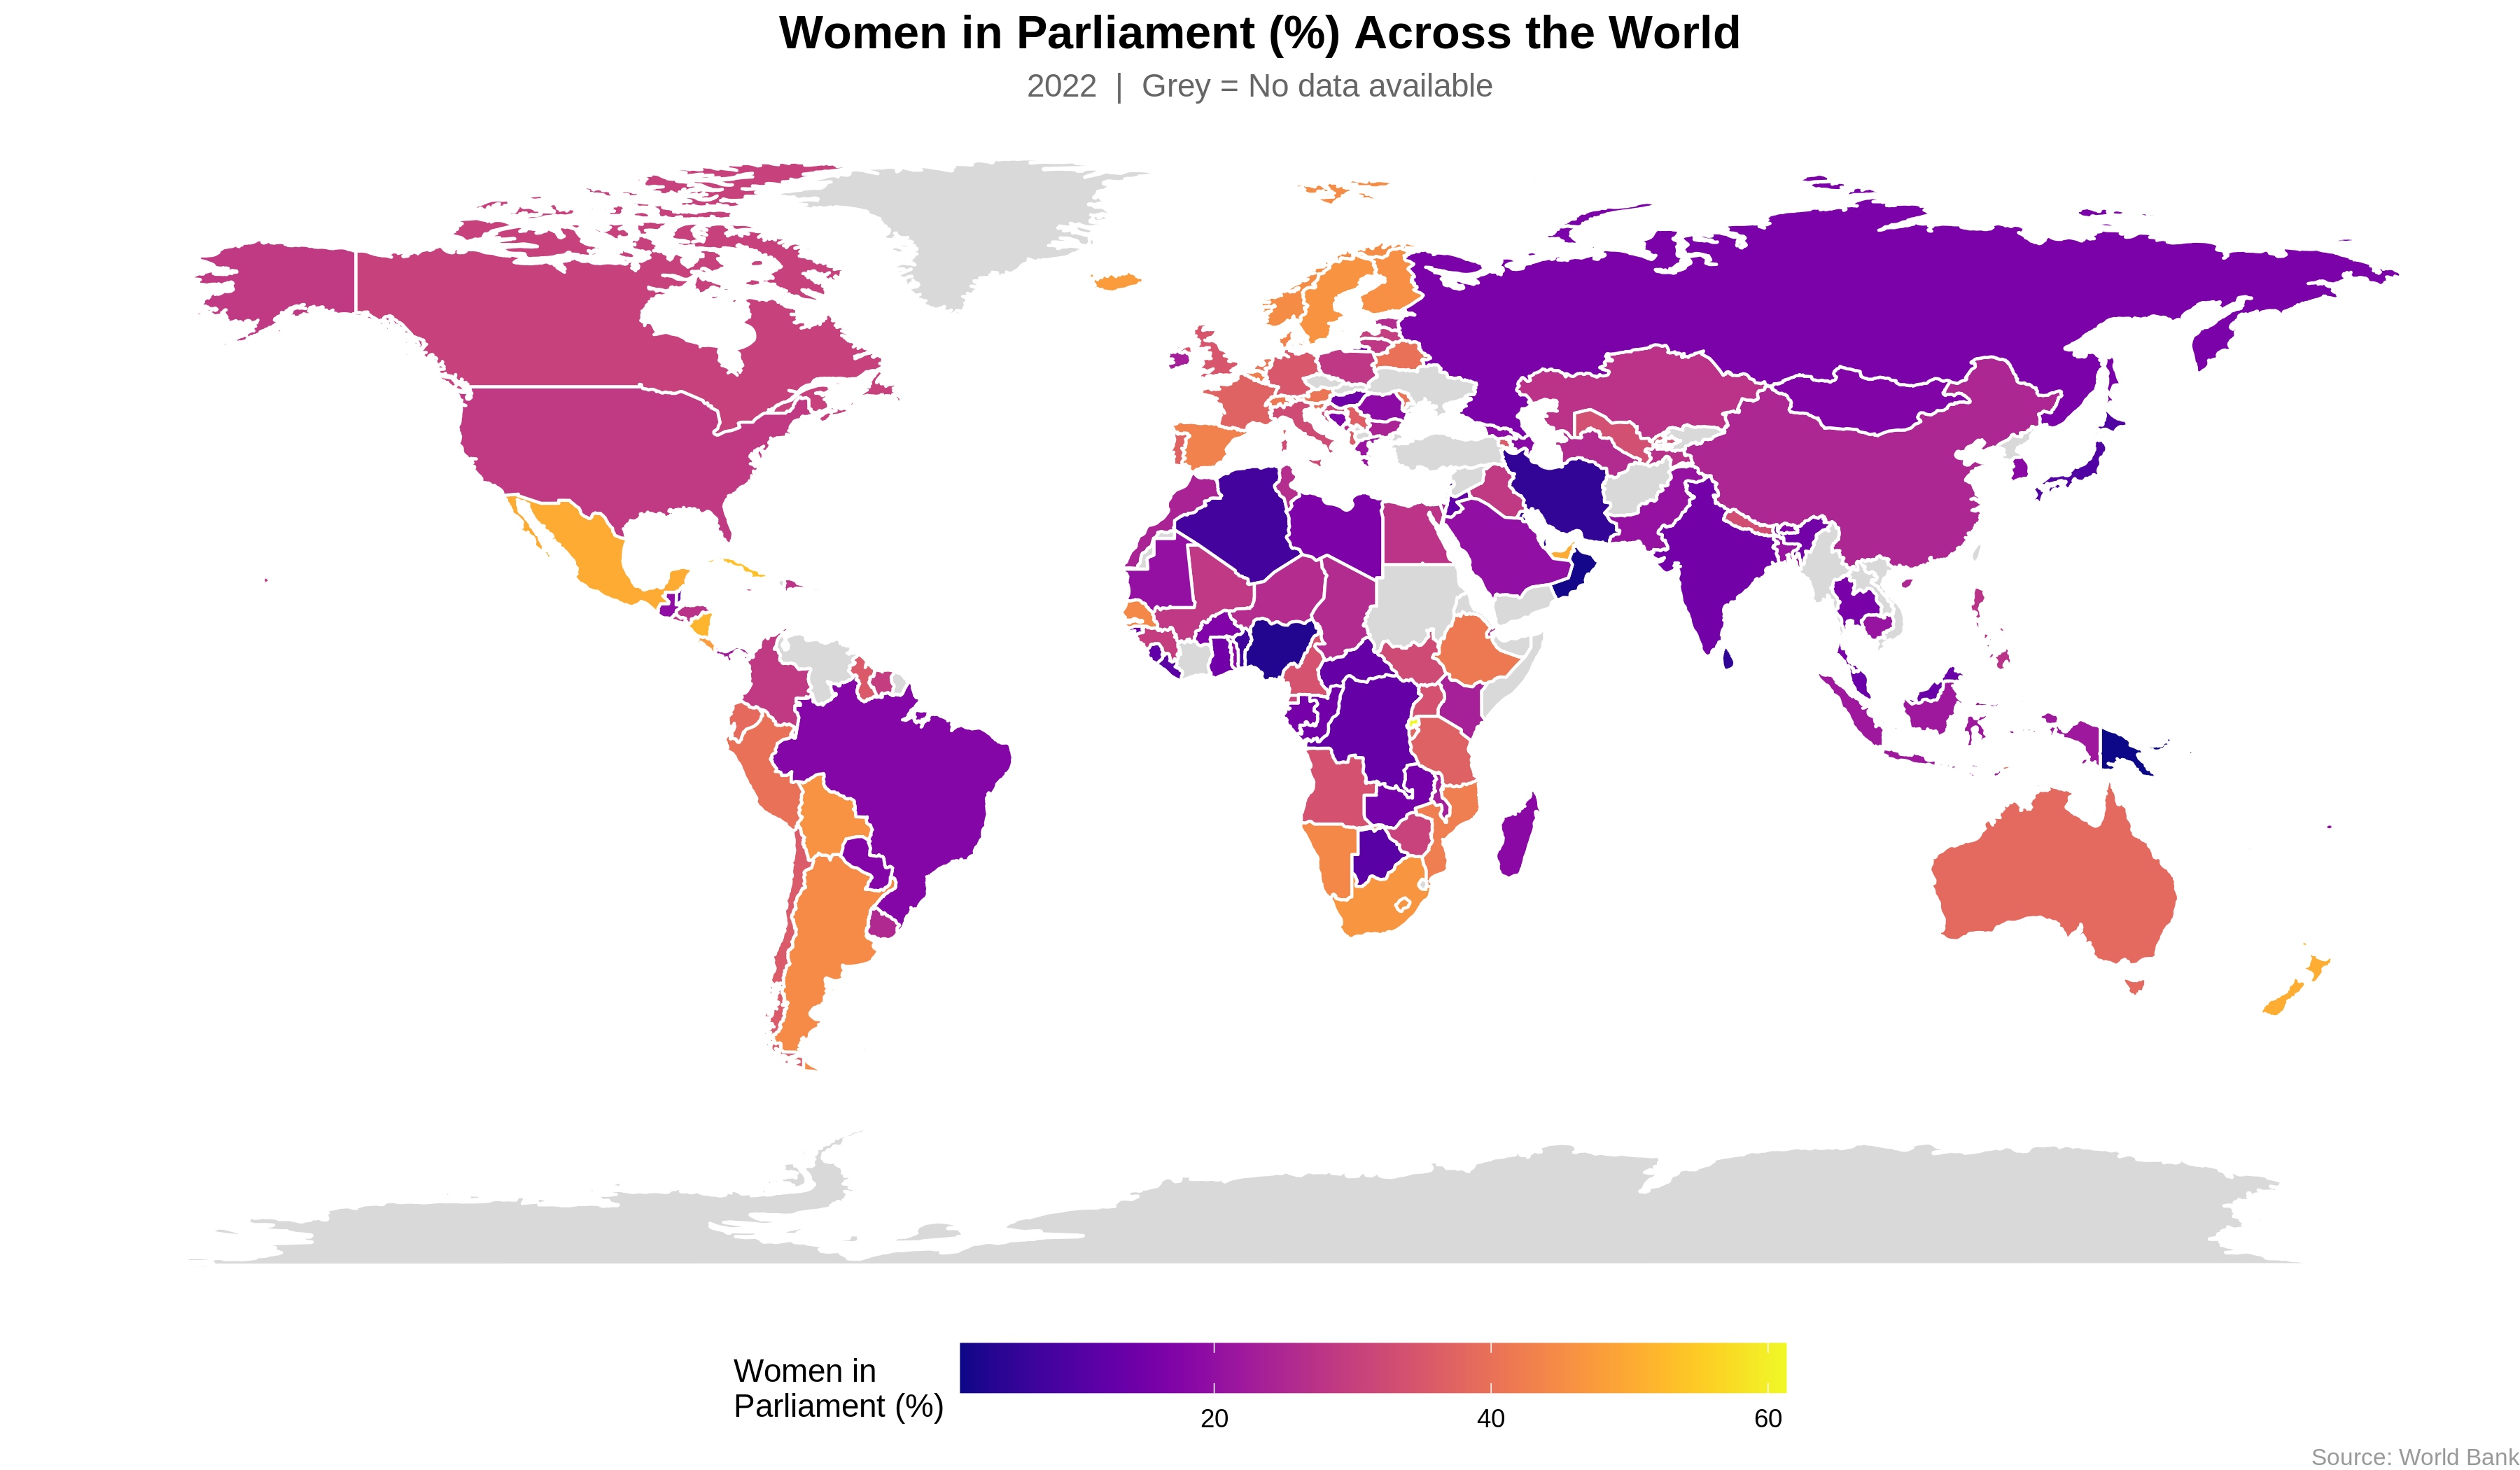
\includegraphics[width=0.95\textwidth]{PS6a_Banerji.png}
    \caption{Women in Parliament (\%) Across the World, 2022}
\end{figure}

\begin{figure}[h]
    \centering
    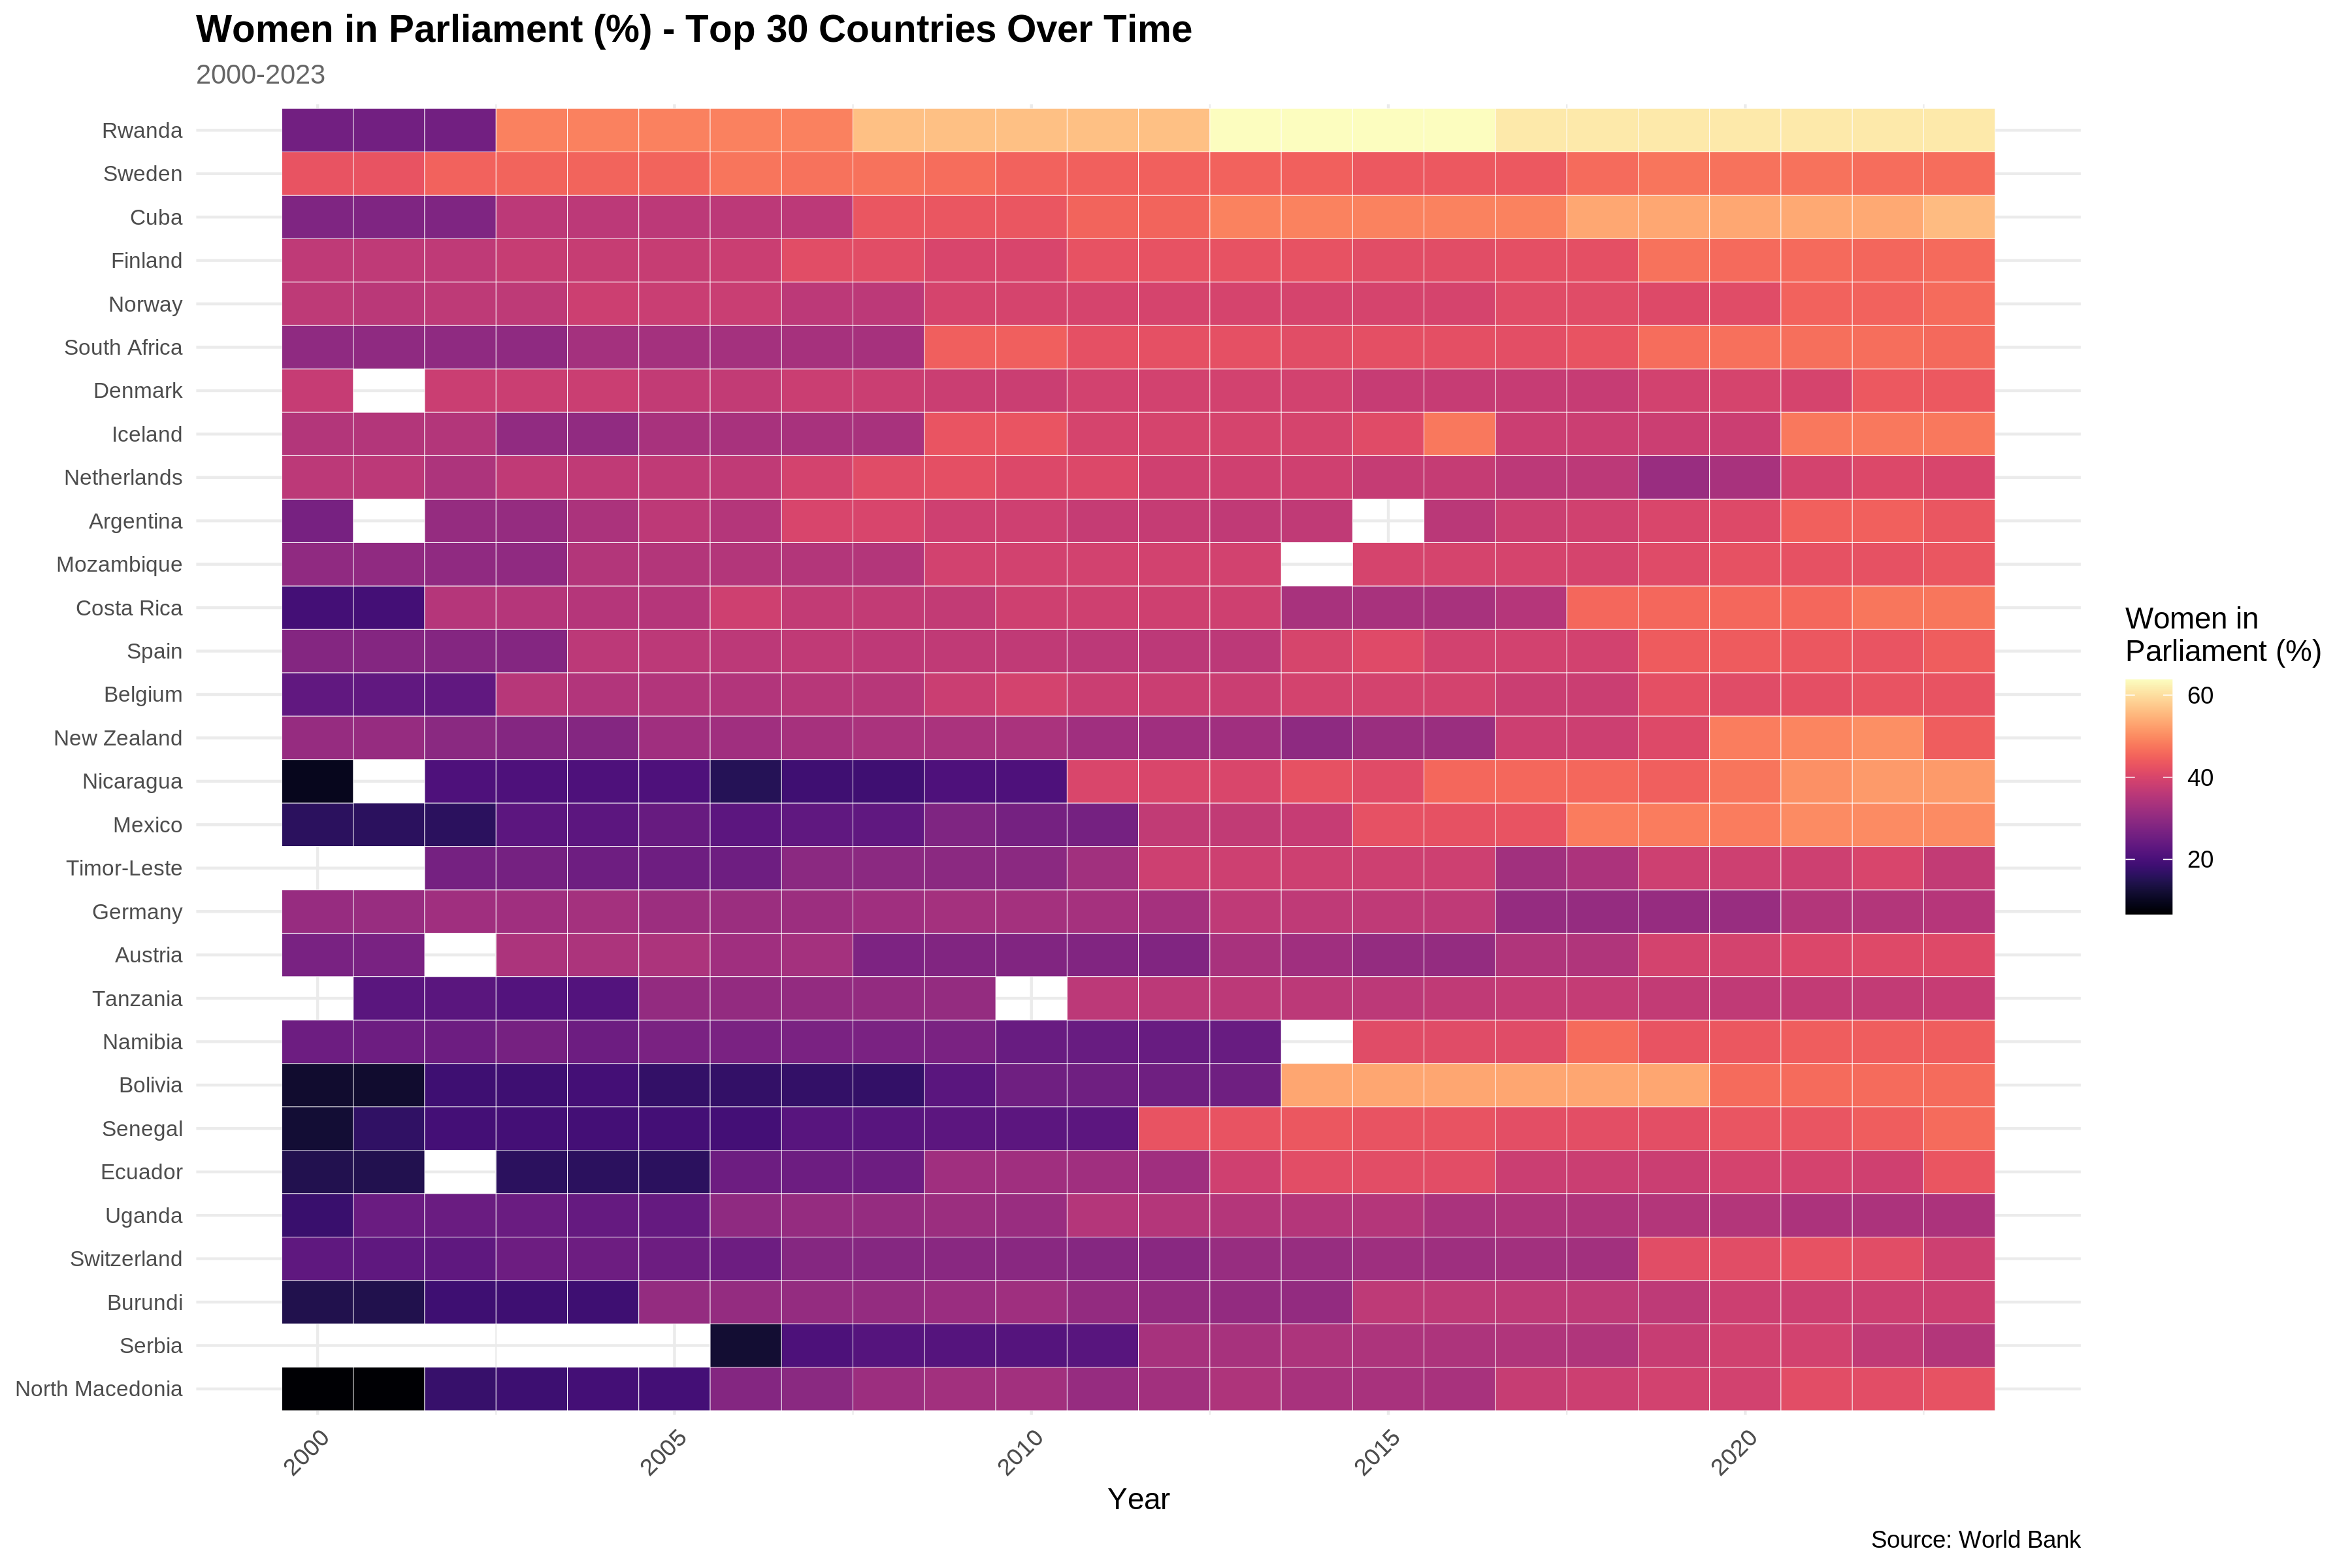
\includegraphics[width=0.95\textwidth]{PS6b_Banerji.png}
    \caption{Heatmap of Women in Parliament (\%) for Top 30
    Countries, 2000--2023}
\end{figure}

\begin{figure}[h]
    \centering
    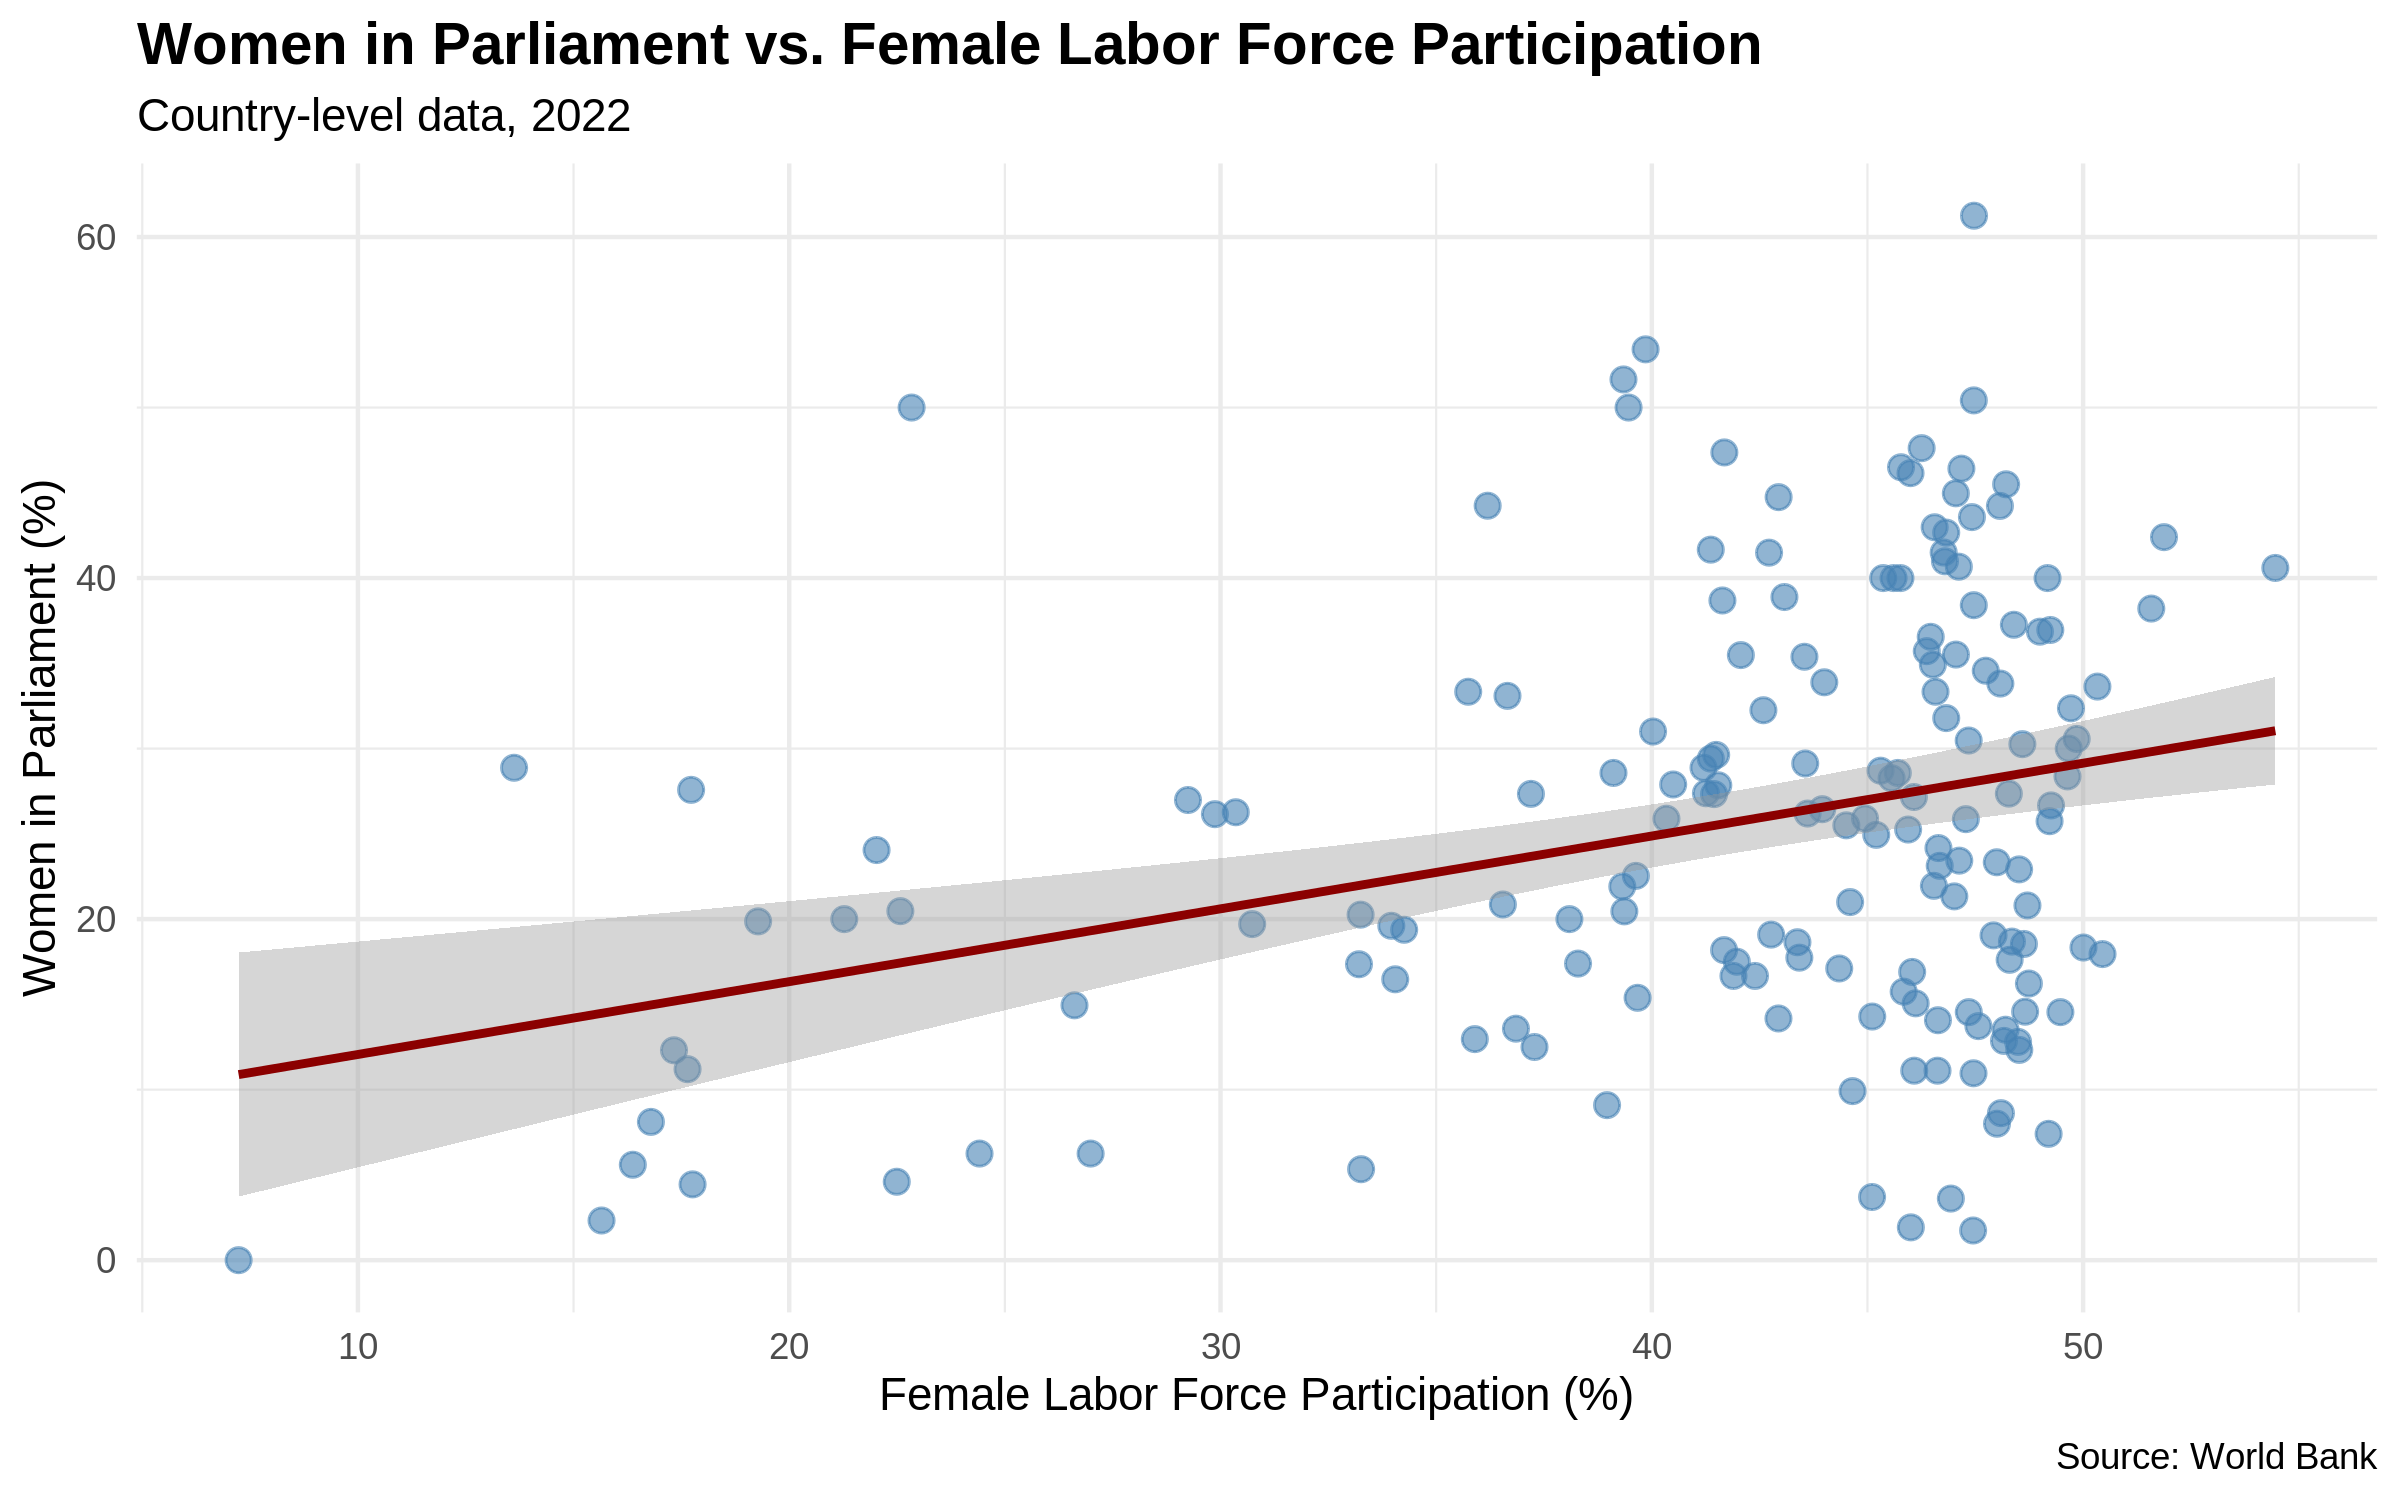
\includegraphics[width=0.95\textwidth]{PS6c_Banerji.png}
    \caption{Women in Parliament (\%) vs. Female Labor Force
    Participation (\%), 2022}
\end{figure}

\section*{Question 5: Explanation of Visualizations}

Figure 1 shows a choropleth world map displaying the percentage of
women in national parliaments across all countries in 2022. Countries
with higher representation appear in brighter colors, while grey
indicates missing data. This reveals strong regional patterns: Nordic
and some African countries tend to have higher female parliamentary
representation, while parts of the Middle East show lower levels.

Figure 2 presents a heatmap of the top 30 countries by average female
parliamentary representation from 2000 to 2023. Each row is a country
and each column is a year. This is useful for identifying trends over
time --- Rwanda stands out with dramatically increasing representation
over the period.

Figure 3 is a scatter plot showing the relationship between female
labor force participation and women in parliament across countries in
2022, with a linear regression line overlaid. The relatively flat
regression line suggests these two measures are not strongly
correlated, indicating that economic participation alone does not
drive political representation.

\section*{Questions 6, 7, and 8}
Files compiled and transferred to OSCER. All required files are
located in \texttt{\textasciitilde/DScourseS26/ProblemSets/PS6/}.
Repository synchronized using \texttt{git add},
\texttt{git commit}, and \texttt{git push origin master}.

\end{document}
